%%%%%%%%%%%%%%%%%%%%%%%%%%%%%%%%%%%%%%%%%%%%%%%%%%%%%%%%%%%%%%%%%
%%%%%%%%%%%%%%%%%%%%%%%%%%%%%%%%%%%%%%%%%%%%%%%%%%%%%%%%%%%%%%%%%
\section{Introduction}\label{sec:expert}
%%%%%%%%%%%%%%%%%%%%%%%%%%%%%%%%%%%%%%%%%%%%%%%%%%%%%%%%%%%%%%%%%
%%%%%%%%%%%%%%%%%%%%%%%%%%%%%%%%%%%%%%%%%%%%%%%%%%%%%%%%%%%%%%%%%
This section is targeted to users who want to differentiated B2.5 themselves in order to add new cost functions, new input parameters to the default list in \ref{sec:tanget_more}, or simply experiment to get to know AD.

The website of Tapenade provides a manual for this tool as well as an extensive set of F.A.Q. \cite{tapesite}.

%%%%%%%%%%%%%%%%%%%%%%%%%%%%%%%%%%%%%%%%%%%%%%%%%%%%%%%%%%%%%%%%%
%%%%%%%%%%%%%%%%%%%%%%%%%%%%%%%%%%%%%%%%%%%%%%%%%%%%%%%%%%%%%%%%%
\section{Running Tapenade in tangent mode}\label{sec:runningTapeTgt}
%%%%%%%%%%%%%%%%%%%%%%%%%%%%%%%%%%%%%%%%%%%%%%%%%%%%%%%%%%%%%%%%%
%%%%%%%%%%%%%%%%%%%%%%%%%%%%%%%%%%%%%%%%%%%%%%%%%%%%%%%%%%%%%%%%%
To start, the user needs to make sure all code changes they need have been correctly implemented and the code has been re-compiled in standalone B2.5 mode, as Tapenade needs the pre-processed source files compiled in:\\
{\tt B2.5/builds/standalone.\${HOST\_NAME}.\${COMPILER}}.\\
Additionally, the environment variable {\tt \$TAPENADEDIR} has to correctly point to the Tapenade installation folder. Be aware that Tapenade requires specific Java installation and that the additional environment variable {\tt \$JAVA\_HOME} must be correctly set, see \cite{tapesite} for details.\\

Once the above requirements have been fulfilled, the user can start differentiating the code. The current implementation requires the user to create the folder:\\
{\tt \$SOLPSTOP/modules/B2.5/build/differentiated\_files.diff\_d}\\
where the compiler will look for the differentiated (diff'ed) source files. The actual differentiation can be done in any other folder/location but then the user has to move the obtained source files to there. From experience, the differentiation failed due to Java memory issues when Tapenade was run on the terminal. As such, it is advised to submit it as a job. In this case, experience with the VSC cluster (Belgium) has shown that 5 processes were apparently needed for successful differentiation, or with enough memory (\(\sim \)10GB). \\

The command line to perform the tangent differentiation is the following:\\
{\tt \$TAPENADEDIR/bin/tapenade -d -O . -head "b2mn\_step(J)/(enepar)"} \\{\tt `collect\_tapenade\_files.sh`}\\
{\tt -ext \$SOLPSTOP/modules/B2.5/src/differentiation/solpsGeneralLib}\\ {\tt  -context -java "-mx30g" -noisize -msglevel 30 -html -r8 >! log}\\
The different options and their meaning is listed below:
\begin{description}
	\item {\tt -d} this flag tells Tapenade to use the tangent AD mode

	\item {\tt -O .} this flag indicates that the output directory is the current directory

	\item {\tt -head "b2mn\_step(J)/(enepar)"} this flag tells Tapenade which is the head/root subroutine for the differentiation and the dependent and independent variables. In the current implementation the head routine should be {\tt b2mn\_step}. Within the first parentheses it is indicated which is/are the dependent variables, i.e. the outputs or cost function $J$. Note that again, in the current implementation, the dependent variable should be $J$. Finally, within the second parentheses are indicated the independent variables, i.e. the input parameters. In this example it is the energy boundary condition parameter, but other common options are the anomalous transport coefficients e.g. {\tt parm\_dna, par\_hce} and {\tt parm\_hci}. Note also that even though these are arrays, it is not necessary to specify which array element, this will be done at a later stage, see section \ref{sec:diff_files}. Finally, be aware that the specified inputs/outputs must be arguments of the head subroutine or must be \textit{visible} within the routine using modules.

	\item {\tt `collect\_tapenade\_files.sh`} this script is run in order to pass to Tapenade the names of the necessary source files to be differentiated. These source files must be the {\tt *.f} and {\tt *.f90} files which have been produced by the CPP preprocessor and this is why the user needs to re-compile the code first.

	\item {\tt -ext \$SOLPSTOP/modules/B2.5/src/differentiation/solpsGeneralLib} this flag provides the description of several functions/subroutines which have been excluded from the differentiation but for which Tapenade needs to know the shape, i.e. number of arguments and their type. Additionally, information on the dependencies between arguments can also be specified. The user is referred to the Tapenade website or manual for additional information.

	\item {\tt -context} this flag allows Tapenade to search dependencies outside the head routine, for example input variables defined within a module. It also introduces some code lines around the head routine which enables verification of derivatives, see section \ref{sec:diff_files}.

	\item {\tt -java "-mx30g"} this flag requires the maximum heap memory for Java to be set to 30 GB. This number came from experience with the code and may change depending on the installation and/or the B2.5 version.

	\item {\tt -noisize} this flag is optional but it is recommended to switch it on. If not, Tapenade will not try to assign the size of newly introduced variables, with the drawback that the user has to do so routine by routine (although the use of a module {\tt DIFFSIZES.F} can partially simplify the procedure). Note that, notwithstanding enabling this option, Tapenade will still not provide the size of few variables. These, for the current implementation, are always found in the same subroutines and as such their size is automatically specified by an ad-hoc script, see section \ref{sec:diff_files}

	\item {\tt -msglevel 30} this flag is optional and controls the amount of output messages that Tapenade issues. It is advised to always use it when the new implementations have been done.

	\item {\tt -html} this flag is optional and asks Tapenade to produce an additional set of {\tt html} files which can be interactively opened with any browser. This allows an easier inspection of the diff'ed subroutines and eventually of errors.

	\item {\tt -r8} this flag is required to specify that the size for reals is 8 bytes (and therefore 16 for double precision reals). See \cite{tapesite} for details.

\end{description}

After a successful differentiation, the output directory will contain the new source files, normally all Fortran .f90 files, which have the same name of the original source files with an additional {\tt \_d}, for example {\tt b2npmo.f} will become {\tt b2npmo\_d.f90}. Within each diff'ed subroutine/module, Tapenade introduces two copies of each subroutine: a diff'ed one, with the additional {\tt \_d} extension in its name, and a non-diff'ed one, with the additional extension {\tt \_nodiff} in its name. Whenever Tapenade finds that a subroutine does not influences any of the dependent or independent variables, then only the {\tt \_nodiff} version is present and used in the diff'ed code. Within each diff'ed subroutine version, variables that have a differentiable influence on the dependent or independent variables are duplicated (both in the subroutine arguments or as local variables), and their name has an additional {\tt d} at the end.\\

Some of the diff'ed files still need some automatized and manual tuning before compilation of the diff'ed code can start, as Tapenade, for example, sometimes misses some arrays dimensioning.\\

Note that also after a successful differentiation Tapenade still issues several hundreds of messages, which should be only warnings. These can normally be ignored as soon as the derivative verification is correct, but the user is encouraged to read the log for certainty.

	%%%%%%%%%%%%%%%%%%%%%%%%%%%%%%%%%%%%%%%%%%%%%%%%%%%%%%%%%%%%%%%%%
	\subsection{Modifications to the tangent differentiated files}\label{sec:diff_files}
	%%%%%%%%%%%%%%%%%%%%%%%%%%%%%%%%%%%%%%%%%%%%%%%%%%%%%%%%%%%%%%%%%
	The next step, before the diff'ed code is compiled, is to modify some of the diff'ed source files to get rid of the small inconsistencies that Tapenade leaves behind and to setup the code such that the derivatives of the input parameter(s) are properly initialized. This procedure has been automatized as much as possible but still some user manual changes are required.\\

	The automatized part is carried out by executing the script {\tt postprocess\_tapenade\_tgt.sh} in the folder \\
	{\tt differentiated\_files.diff\_d}, where the diff'ed files should be moved after differentiation (keep the original diff'ed files for backup). This scripts performs different actions on specific source files (more details can be found in \ref{script_ad}). It is likely that with new code developments or new Tapenade versions, some of such modifications are not necessary anymore and new ones can arise. Therefore the user is invited to look at the script file description and at the script itself in case new modifications should be necessary.\\

	The automatized part will perform the following actions, which the user can take inspiration from for personal needs:
	\begin{itemize}

		\item Initialize the diff'ed input parameter(s) in routine {\tt b2mn\_d.F90}. This step depends on which input parameters have been selected as independents, and a few examples are given below:
		\begin{description}
			\item[\tt enepar] If the user wants the derivatives wrt the energy boundary condition parameter, for example at the core, the target variable is {\tt enepar(1,1)} (note that this would also be the variable that the user would need to perturb when doing finite differences). Therefore the two following lines can be inserted just before the call to {\tt b2mn\_step\_d}:\\
			{\tt enepard = 0.0\_R8}\\
			{\tt enepard(1,1) = 1.0\_R8}

			\item[\tt parm\_hce] In case the user wants the derivative wrt the anomalous electron heat diffusion coefficient $\chi_{\perp,e}$, the target variable is {\tt parm\_hce}. Therefore the following line can be inserted just before the call to {\tt b2mn\_step\_d}:\\
			{\tt parm\_hced = 1.0\_R8}

			\item[\tt parm\_dna] The case of the derivative wrt the anomalous (density driven) particle diffusion coefficient $D_{\perp}$ is similar as for {\tt parm\_hce}. The target variable is {\tt parm\_dna(is)} and the initialization, to be placed again just before the call to {\tt b2mn\_step\_d}:\\
			{\tt parm\_dnad = 0.0\_R8}\\
			{\tt parm\_dnad(1) = 1.0\_R8} (in case the target is species 1)
		\end{description}

		\item Obtain in output the cost function gradient. The script modifies {\tt b2mndr\_1\_d} within {\tt b2mod\_driver\_diff.F90}. Right after the call to {\tt b2usr\_cost\_function\_d}, the cost function value is printed in a for-loop, and just after that a few new lines are added to print in the log tile the cost function gradient.
	\end{itemize}


	This script does not guarantee a 100\% success, as changes in the code may affect how Tapenade writes the diff'ed source files. Thus, the user is encouraged to look into the diff'ed files and modify according to their needs.

	If the user wants to verify the obtained derivatives using the Tapenade built-in option, then no automatic initialization of the diff'ed input parameters should be done. Also, the user needs to re-introduce code sections in {\tt b2mn\_d} around the call to {\tt b2mn\_step\_d} which the script will have removed (thus useful to keep the original files). These start with {\tt CALL ADCONTEXTTGT\_*} and automatically initialize the input parameters for verification. More details on this procedure are available in \cite{tapesite}.

	%%%%%%%%%%%%%%%%%%%%%%%%%%%%%%%%%%%%%%%%%%%%%%%%%%%%%%%%%%%%%%%%%
	\subsection{Tangent code compilation}
	%%%%%%%%%%%%%%%%%%%%%%%%%%%%%%%%%%%%%%%%%%%%%%%%%%%%%%%%%%%%%%%%%
	Having completed the modifications to the diff'ed source files, the compilation can be carried out. To do so, the user has to first define the environment variable:\\
	{\tt \$ setenv DIFF\_D yes}  or simply use the alias {\tt set\_d}\\
	and then make the objects and dependencies list in the standard way in {\tt \$SOLPSTOP}:\\
	{\tt \$ gmake listobj depend}\\
	Finally, the diff'ed code compilation can be started with the command:\\
	{\tt \$ gmake b25\_diff\_d}\\

	In case the {\tt debug} version is needed, it follows the standard {\tt SOLPS-ITER} rules which simply require to append {\tt \_debug} to the make targets.


	%%%%%%%%%%%%%%%%%%%%%%%%%%%%%%%%%%%%%%%%%%%%%%%%%%%%%%%%%%%%%%%%%
	\subsection{Tangent vector mode}\label{sec:tgtvec}
	%%%%%%%%%%%%%%%%%%%%%%%%%%%%%%%%%%%%%%%%%%%%%%%%%%%%%%%%%%%%%%%%%
	If one wants to obtain the full Jacobian, i.e. the gradient with respect to all (ar at least several) input parameters, Tapenade provides this feature through the so-called vector or multi-directional tangent mode. This is also the correct option that enables optimization of multiple parameter using tangent AD.
	To do so, the user should insert the flag {\tt -multi}  and specify different independents when invoking the Tapenade command line described in section \ref{sec:runningTapeTgt}, which for example can be modified as follows:\\
	{\tt -multi -head "b2mn\_step(J)/(enepar enipar parm\_dna parm\_hci parm\_hce)"} \\
	In this way Tapenade will provide the derivative of all cost functions {\tt J} against the five input parameters specified (the ordering does not matter).
	The procedure to follow is very similar to the one described before, with some slight modifications.

	The first difference wrt to the normal tangent AD mode is that now the diff'ed source files and routines have a different naming, using {\tt \_dv} instead of {\tt \_d}, and {\tt \_diffv} instead of {\tt \_diff} for modules. Additionally, the diff'ed variables have now an extra dimension, which is the derivative direction. For example a variable which had primal size {\tt (1:nCv,0:ns-1)} now has dimensions {\tt (nbdirsmax,1:nCv,0:ns-1)}. The extra dimension maximum size {\tt nbdirsmax} can be defined in two ways: either by the use of a new module {\tt DIFFSIZES.F}, which is automatically placed by Tapenade in each routine (default option); or by differentiating using the additional command line option {\tt -nbdirsmax \#}, with {\tt \#} the maximum number of directions (in our example 5, as the number of input parameters, for example). The first method however, allows more flexibility in the sense that if the dependents are themselves arrays (as in the case shown above), the user can choose to obtain the derivative wrt all the elements of such arrays. Finally, each routine has now an additional argument, {\tt nbdirs}, which defines the actual number of directions over which calculating the derivative. This parameter is therefore used in additional {\tt DO}-loops at the lowest/innermost level. It is thus clear that the computational cost now scales with the number of actual directions computed {\tt nbdirs}. This has to be defined at the start of  {\tt b2mn\_d.F90} and must of course be smaller or equal to {\tt nbdirsmax}.\\

	Tangent vector mode requires scripts similar to those for the normal tangent mode, but their principles remain the same. Therefore, the user can follow the same procedure described in section \ref{sec:diff_files}, this time executing the script {\tt postprocess\_tapenade\_tgt\_multi.sh} in the directory {\tt differentiated\_files.diff\_d}. This will:
	\begin{itemize}

		\item initialize in {\tt b2mn\_d.F90} the variable {\tt nbdirs} to a specific default integer. This must be done before calling the fist subroutine ({\tt b2mn\_init\_dv})

		\item initialize the diff'ed input parameters.They have now an extra first dimension, that must not clash with the other parameters. For the default example provided this means:
		\begin{description}
			\item{enepard(1,1,1) = 1.0\_R8}
			\item{enipard(2,1,1) = 1.0\_R8}
			\item{parm\_hced(3) = 1.0\_R8}
			\item{parm\_hcid(4,1) = 1.0\_R8}
			\item{parm\_dnad(5,1) = 1.0\_R8}
		\end{description}
		In this way, the first direction will evaluate the cost function gradient wrt {\tt enepar(1,1)}, the second wrt {\tt enipar(1,1)}, and so on. It is instead WRONG to initialize this way: {\tt enepard(1,1,1) = 1.0\_R8}	and {\tt parm\_hced(1) = 1.0\_R8}. In this case the first derivative direction would yield the sum $\frac{\partial J}{\partial enepar} + \frac{\partial J}{\partial cfhce}$

		\item Modify the printout of the cost function gradient in {\tt b2mod\_driver\_diffv.F90} after the call to \\{\tt b2usr\_cost\_function\_dv}. In case of errors, the user needs to wrap the {\tt DO}-loop with the additional loop on {\tt nbdirs} and modify the printout such that {\tt Jd(idir,icf)} is correctly addressed

		\item Change the use of module {\tt DIFFSIZES} into {\tt b2mod\_diffsizes}, and create such module
	\end{itemize}

	Compilation and running of the multidirectional tangent mode work the same as for the normal mode.


	\subsection{Enabling output of differentiated quantities}\label{sed:diffout}
	It is possible to enable additional output to check the convergence of the diff'ed equations through their residuals. Unfortunately, Tapenade does not automatically introduce diff'ed code that mimics the same output of the primal quantities, e.g. the residuals or the time traces. Therefore, the script {\tt postprocess\_tapenade\_tgt\_multi.sh} automatically introduces some new calls to routines.

	\paragraph{Residuals output}
	For the output of the diff'ed equation residuals an additional file {\tt b2ftraced} needs to be written and the dedicated quantities calculated. For this purpose, three dedicated subroutines from B2.5 have been adapted and are available in {\tt B2.5/src/differentiation}: {\tt b2mwqt\_diff.F}, {\tt b2mxac\_diff.F} and {\tt b2mxar\_diff.F}. Such routines are automatically copied into the {\tt differentiated\_files.diff\_d} folder. Additionally, the script brings changes in the following routines:
	\begin{description}
		\item[\tt b2mndt\_d.F90] The first change deals with declaration of diff'ed residuals variables, while  other two the above mentioned routines are called to evaluated the norm of the residuals and of the corrections and to write the output in {\tt b2ftraced}. Compare with the unmodified output of Tapenade or with \\{\tt src/differentiation/tangent/b2mndt\_dv.F90} if help is needed.

		\item[\tt b2mod\_main\_diff.F90] An extra line that opens the {\tt b2ftraced} file is added.

		\item[\tt b2mod\_driver\_diff.F90] A line that calls the {\tt createB2Diagnostic} subroutine is added.

		\item[\tt b2mnds\_d.F90] Headers are written to {\tt b2ftraced} file

%		\item[\tt b2mod\_residuals\_diff.F90] Look in the file for the three labels and uncomment the lines following them. The first one refers to declaration of diff'ed residuals variables, the second to their allocation and initialization, and the third to their de-allocation. The first set of commented line is somehow moved by Tapenade within the {\tt CONTAINS} statement, and therefore has to be placed before it

%		\item[\tt b2mod\_diag\_diff.F90] Look in the file for the three labels and uncomment the lines following them. The first one refers to declaration of diff'ed residuals per region variables, the second to their allocation and initialization, and the third to their de-allocation.
	\end{description}
	Note: it can be that the source code of these routines needs to be further modified for the user needs or if developments are made in the original routines.

	\paragraph{Time traces output}
	This feature is not yet available

	\subsubsection{Enabling reading and writing of differentiated state file}
	It is possible to also enable the reading/writing of a differentiated plasma state file, so that it is possible to continue a run using the diff'ed code without re-starting from zero the derivative part. This however is not the standard behaviour of the tangent or adjoint code found in the source files!\\
	 Here a clarification has to be made, because with the diff'ed code it is anyway possible to continue a run in the 'standard' way, by copying {\tt b2fstate} into {\tt b2fstati} and letting the primal quantities converge. On the other hand, the derived quantities do not have an initial state file, and therefore always restart from a flat {\tt 0.0}. This might not be a problem in general, but in cases with large grids and/or with long convergence rate of the primal (e.g. with drifts), it is desirable to be able to save the state of the derived quantities and continue from it. Therefore two additional files can be introduced specifically for the diff'ed code (they are not needed for the standard B2.5 simulations): {\tt b2fdiffi} and {\tt b2fdiffe}. The first is the initial diff'ed plasma state and the second is the final diff'ed plasma state. Therefore, to continue a run with the diff'ed code, the user can copy {\tt b2fstate} into {\tt b2fstati} and {\tt b2fdiffe} into {\tt b2fdiffi}. The initial diff'ed state file must be present in the run directory even if reading/writing of diff'ed state files is not enabled (it is a dependency in the runs Makefile), and if not yet available the user can simply use {\tt b2fstati}.\\

	To enable this code option, two dedicated subroutines from {\tt b2us\_plasma\_state.F} have been adapted and are available in {\tt B2.5/src/differentiation}: {\tt read\_plasma\_state\_diff.F} and {\tt write\_plasma\_state\_diff.F}. Such routines are automatically copied into the {\tt differentiated\_files} folder. Additionally, the user has manually add lines in the following routines:
	\begin{description}
		\item[\tt b2mod\_main\_diff.F90] Action is needed to first open the {\tt b2fdiffi} file and reads the file version. Here the user is encouraged to also modify the lines that follow, where the file version {\tt b2fdiffi\_version} should be added to the comparison. Further, headers from {\tt b2fdiffi} should be read and some quantities tested, then a new {\tt b2fdiffe} file should be opened. Compare and mimic how {\tt b2fstati} and {\tt b2fstate} are handled

		\item[\tt b2mod\_driver\_diff.F90] Action is needed to enable the call to {\tt read\_plasma\_state\_diff} and \\{\tt write\_plasma\_state\_diff} respectively, again mimicking how the state plasma is read/written

		\item[\tt b2mnds\_d.F90] Action is first to re-enble the statement function {\tt ltst}, which is needed afterwards. At second, the headers of {\tt b2fdiffi} should be read and tested. At third the label of {\tt b2fdiffi} should be printed in output. Finally at fourth, headers should be written to  {\tt b2fdiffe}. Again, compare and mimic how {\tt b2fstati} and {\tt b2fstate} are handled
	\end{description}
	Note: it can be that the source code of these routines needs to be further modified for the user needs or if developments are made in the original routines.



	\paragraph{IMPORTANT NOTE FOR VECTOR MODE}
	The output of differentiated quantities is available only for the first direction for the multidirectional mode. Further developments will allow complete output of all directions.

	The residuals output follows what has been described in section \ref{sed:diffout}. Three dedicated subroutines from B2.5 have been adapted and are available in {\tt B2.5/src/differentiation}: {\tt b2mwqt\_diffv.F}, {\tt b2mxac\_diffv.F} and {\tt b2mxar\_diffv.F}. Such routines are automatically copied into the {\tt differentiated\_files.diff\_d} folder. The script provide modifies the same lines in the routines described in section \ref{sed:diffout}.

	READING AND WRITING OF DIFF'ED STATE FILES FOR VECTOR MODE IS NOT YET DEVELOPED

%%%%%%%%%%%%%%%%%%%%%%%%%%%%%%%%%%%%%%%%%%%%%%%%%%%%%%%%%%%%%%%%%
%%%%%%%%%%%%%%%%%%%%%%%%%%%%%%%%%%%%%%%%%%%%%%%%%%%%%%%%%%%%%%%%%
\section{Running Tapenade in adjoint mode}\label{sec:runningTapeAdj}
%%%%%%%%%%%%%%%%%%%%%%%%%%%%%%%%%%%%%%%%%%%%%%%%%%%%%%%%%%%%%%%%%
%%%%%%%%%%%%%%%%%%%%%%%%%%%%%%%%%%%%%%%%%%%%%%%%%%%%%%%%%%%%%%%%%
Again, the user needs to make sure all code changes they need have been correctly implemented. Specifically for adjoint AD, the time-iterating scheme of B2.5 (essentially a for-loop on the number of iterations) needs to be converted into a fixed-point iterator form. This is essential to apply the \textit{two-phases} scheme, which allows significantly lower memory requirements, see \cite{carlijcp,griewank}. To convert into a fixed point form, users need to set a specific environment variable and recompile {\tt b2mod\_driver}:
\begin{description}
	\item 	{\tt \$ setenv FIXED\_POINT yes}
	\item 	{\tt \$ touch \$SOLPSTOP/modules/B2.5/src/driver/b2mod\_driver.F}
	\item 	{\tt \$ gmake b25}
\end{description}

After that, the user should create the folder:\\
{\tt \$SOLPSTOP/modules/B2.5/build/differentiated\_files.diff\_b}\\
(note the different ending compared to tangent mode!) where the compiler will look for the adjoint diff'ed source files. For adjoint AD the time required for differentiation is much longer (5 hours instead of 1 on the VSC cluster in Belgium). Again, experience with VSC shows that 5 processes are needed for successful differentiation, or about 10 GB of memory. \\

The command line to perform the adjoint differentiation is the following:\\
{\tt \$TAPENADEDIR/bin/tapenade -b -O . -head "b2mndr\_1(J)/(parm\_dna parm\_hce}\\
{\tt parm\_hci enepar enipar conpar)" `collect\_tapenade\_files.sh` -ext}\\
{\tt \$SOLPSTOP/modules/B2.5/src/differentiation/solpsGeneralLib -context -java}\\
{\tt "-mx30g" -noisize -msglevel 30 -html -r8 >! log}\\

The options are the same as for tangent AD with the difference only in the flag {\tt -b} which enables adjoint mode. \textbf{Important!} note the different head routine, which for adjoint is {\tt b2mndr\_1}!

As with tangent mode, new source files are produced by Tapenade, this time with {\tt \_b} in place of {\tt \_d} for files, routines, and variables names. Modules keep the same {\tt \_diff} naming convention. Similarly as with tangent AD, diff'ed files needs some tuning, described in the following section.

	%%%%%%%%%%%%%%%%%%%%%%%%%%%%%%%%%%%%%%%%%%%%%%%%%%%%%%%%%%%%%%%%%
	\subsection{Modifications to the differentiated files}\label{sec:diff_files_adj}
	%%%%%%%%%%%%%%%%%%%%%%%%%%%%%%%%%%%%%%%%%%%%%%%%%%%%%%%%%%%%%%%%%
	An automatized correction of the diff'ed files is carried out now by executing the script {\tt postprocess\_tapenade\_adj.sh} in the folder {\tt differentiated\_files.diff\_b}. As with tangent mode, new code developments may make some of the script actions obsolete or insufficient, and the user should then manually tune the required files.

	The automatized part will perform the following actions, which the user can take inspiration from for personal needs:
	\begin{itemize}

		\item Initialize the diff'ed output parameter(s) in routine {\tt b2mn\_step\_b} within {\tt b2mod\_main\_diff.F90}. This step depends on which output parameters have been selected as dependents, and the suggested default is the cost function {\tt J}. In this case, the initialization should be done just before the call to {\tt b2mndr\_1\_b} in the following way:\\
		{\tt jb = 0.0\_R8}\\
		{\tt jb(1) = 1.0\_R8}\\
		This is because the optimization (see section \ref{sec:optimization}) will only employ the first element of the cost function array {\tt J}.

		\item Obtain in output the cost function gradient. The script modifies {\tt b2mn\_step\_b} and also {\tt b2mndr\_1\_b} within {\tt b2mod\_driver\_diff.F90}, to print the gradient at each iteration. A few examples are are:\\
		{\tt write(*,*) 'GRADIENT conpar 1',conparb(1,1,1)}, for continuity BC at boundary 1, species 1\\
		{\tt write(*,*) 'GRADIENT conpar 2',conparb(0,2,1)}, for continuity BC at boundary 2, species 0\\
		{\tt write(*,*) 'GRADIENT enepar 1',eneparb(3,1)}, for electron energy BC at boundary 3\\
		{\tt write(*,*) 'GRADIENT dna ',parm\_dnab(1)}, for $D_\perp$, species 1\\
		{\tt write(*,*) 'GRADIENT hce ',parm\_hceb}	, for $\chi_{e,\perp}$
	\end{itemize}


	Again, if the user wants to verify the obtained derivatives using the Tapenade built-in option, then no automatic initialization should be done and the calls to {\tt CALL ADCONTEXTADJ\_*} need to be re-introduced in {\tt b2mn\_step\_b} within {\tt b2mod\_main\_diff.F90} around the call to {\tt b2mndr\_1\_b}.

	A simple modification of the {\tt while} loop condition in {\tt b2mndr\_1\_b} enables the user to stop the fixed point iterator after the required number of iterations, by automatically modifying {\tt b2mndr\_1\_b} to have the following:\\
	{\tt DO WHILE ((res\_max .GE. res\_quit) .and. (itim .le. ntim))}\\
	{\tt DO WHILE ((cumul .GT. res\_quit) .and. (ITERCOUNT.le.ntim))}\\

	\textbf{Note} It should be possible to re-enable the elapsed time  and .quit options to smoothly stop the adjoint code, but this has not been done yet.

	%%%%%%%%%%%%%%%%%%%%%%%%%%%%%%%%%%%%%%%%%%%%%%%%%%%%%%%%%%%%%%%%%
	\subsection{Adjoint code compilation}
	%%%%%%%%%%%%%%%%%%%%%%%%%%%%%%%%%%%%%%%%%%%%%%%%%%%%%%%%%%%%%%%%%
	Having completed the modifications to the diff'ed source files, the compilation can be carried out. To do so, the user has to first define the environment variable:\\
	{\tt \$ setenv DIFF\_B yes}  or simply use the alias {\tt set\_b}\\
	and then make the objects and dependencies list in the standard way in {\tt \$SOLPSTOP}:\\
	{\tt \$ gmake listobj depend}\\
	Finally, the diff'ed code compilation can be started with the command:\\
	{\tt \$ gmake b25\_diff\_b}\\

	In case the {\tt debug} version is needed, it follows the standard {\tt SOLPS-ITER} rules which simply require to append {\tt \_debug} to the make targets.

	%%%%%%%%%%%%%%%%%%%%%%%%%%%%%%%%%%%%%%%%%%%%%%%%%%%%%%%%%%%%%%%%%
	\subsection{Enabling output of differentiated quantities}
	%%%%%%%%%%%%%%%%%%%%%%%%%%%%%%%%%%%%%%%%%%%%%%%%%%%%%%%%%%%%%%%%%
	Currently it hasn't been tested if additional outputs like residuals or saving/reading an initial adjoint derivative state file is possible.

	Also, if one for example wants to obtain a full 2D map of transport coefficient sensitivity (e.g. for {\tt dna0} which is defined on each cell), either some manual tuning of {\tt b2tqna\_b} is necessary to save {\tt cfdnab} before is re-set to zero, or the differentiation command should probably include as additional independent {\tt cfdna}. An example of the first method is included in the current source files for {\tt B2.5/src/differentiation/adjoint}

	%%%%%%%%%%%%%%%%%%%%%%%%%%%%%%%%%%%%%%%%%%%%%%%%%%%%%%%%%%%%%%%%%
	\subsection{AD pragmas}
	%%%%%%%%%%%%%%%%%%%%%%%%%%%%%%%%%%%%%%%%%%%%%%%%%%%%%%%%%%%%%%%%%
	Some AD pragmas are already inserted as comments in the B2.5 code and mainly affect the adjoint mode. Such pragmas are:
	\begin{description}
		\item[AD FP-LOOP ``state''] This pragma is used in {\tt b2mndr\_1} to tell Tapenade that the loop that follows is a fixed point iterator, with state variable "state". It is required for efficient memory usage in adjoint mode and is not relevant for tangent mode.
		\item[AD NOCHECKPOINT] This pragma is used at the beginning of several low-level routines. In adjoint mode it turns off checkpointing of this routine (i.e. saving a snapshot of the variables around the call to this routine), which at the low level of the call tree may be less performing than full recalculation
		\item[AD II-LOOP] This pragma indicates that the following loop has independent iterations, which means that adjoint AD can perform better computations by applying an ad-hoc checkpointing scheme. Seems to have sped-up the adjoint code when used for the matrix computation in {\tt b2usco, b2usmo, b2uspo, b2usht}.
	\end{description}

%%%%%%%%%%%%%%%%%%%%%%%%%%%%%%%%%%%%%%%%%%%%%%%%%%%%%%%%%%%%%%%%%
%%%%%%%%%%%%%%%%%%%%%%%%%%%%%%%%%%%%%%%%%%%%%%%%%%%%%%%%%%%%%%%%%
\section{Pre-processing mode}
%%%%%%%%%%%%%%%%%%%%%%%%%%%%%%%%%%%%%%%%%%%%%%%%%%%%%%%%%%%%%%%%%
%%%%%%%%%%%%%%%%%%%%%%%%%%%%%%%%%%%%%%%%%%%%%%%%%%%%%%%%%%%%%%%%%
Tapenade allows a pre-processing mode in which basically it parses through the source files but do not attempt to write any derivative information. The output is just the original code but written out by Tapenade in F90 style. This Tapenade mode is quite useful and quick to test if a certain cost function depends on certain parameters, to check for potential errors in the code (see common pitfalls \ref{sec:errors_ad}), and to test compilation of the diff'ed files and verify that the outcome is the same of the original code.

The command line to perform the pre-processing mode is the following:\\
{\tt \$TAPENADEDIR/bin/tapenade -p -O . -head "b2mn\_step(J)/(parm\_dna parm\_hce}\\
{\tt parm\_hci enepar enipar conpar)" `collect\_tapenade\_files.sh` -ext}\\
{\tt \$SOLPSTOP/modules/B2.5/src/differentiation/solpsGeneralLib -context -java}\\
{\tt "-mx30g" -noisize -msglevel 30 -html -r8 >! log}\\

The only difference wrt to tangent and adjoint mode is in the flag ``{\tt -p}'' in place of ``{\tt -d}'' or ``{\tt -b}''.

%%%%%%%%%%%%%%%%%%%%%%%%%%%%%%%%%%%%%%%%%%%%%%%%%%%%%%%%%%%%%%%%%	%%%%%%%%%%%%%%%%%%%%%%%%%%%%%%%%%%%%%%%%%%%%%%%%%%%%%%%%%%%%%%%%%
\section{Common pitfalls}\label{sec:errors_ad}
%%%%%%%%%%%%%%%%%%%%%%%%%%%%%%%%%%%%%%%%%%%%%%%%%%%%%%%%%%%%%%%%%
%%%%%%%%%%%%%%%%%%%%%%%%%%%%%%%%%%%%%%%%%%%%%%%%%%%%%%%%%%%%%%%%%

In case of an unsuccessful differentiation, at the end of the log file produced by Tapenade it will appear a line stating "Differentiation failed". In this case, no new source files will be present in the output directory and the user will need to look into the log file for errors.

From experience, the differentiation failure was caused by these main aspects:
\begin{itemize}
	\item Presence of {\tt entry} statements. These are not tolerated by Tapenade and therefore an error message from the Fortran parser is issued in the log file. Therefore, some subroutines have been excluded from the differentiation or have been restructured to become a module.

	\item NetCDF routines. All the NetCDF routines have therefore been moved to a single module, which is then excluded from the differentiation. These routines have also been described in \\{\tt B2.5/src/differentiation/solpsGeneralLib} so that Tapenade knows their shape.

	\item Statement functions. Although generally accepted by Tapenade, they have caused problems in two ways. First, because Tapenade expects them to be defined after all variables declaration. Second, because sometimes such statement functions use variables which are also used within the subroutine/function. While in the first case the Fortran parser will issue an error and the differentiation will fail, in the second case the differentiation will succeed but the derivatives might be incorrect. Therefore, when possible these statement functions have been substituted by normal functions.
\end{itemize}

The items above were the main cause of error in the differentiation but the user is encouraged to always verify the quality of the derivative information using finite differences or the built-in verification procedure produced by the {\tt -context} flag.\\

Other errors encountered:
\begin{itemize}
	\item Some labels of the {\tt GOTO} statements in {\tt b2stbc\_phys.F} were disappearing in the diff'ed file. Therefore, all these statements have been replaced by {\tt SELECT CASE}. This has solved the problem, which seems to arise only when many {\tt GOTO}'s are present.

	\item Several other 'small' errors in the differentiation are still present and are addressed in the next section by the scripts described there. These are mostly related to formatting and to the fact that some subroutines have been excluded from Tapenade, while in fact they do not prevent correct propagation of the derivative information.

	\item ALIASING: it is a bad coding practice which is normally (but apparently not always) spotted by Tapenade in the log file. It is a quite important issue for adjoint AD, while is not a problem for tangent. The explanation of the potential error comes from the example in Figure \ref{fig_alias}. The function{\tt fun} and its call are on the left of the figure, while the adjoint af the function {\tt fun\_b} and its call are on the right.
	\begin{figure}[h]
		\centering
		\subfigure{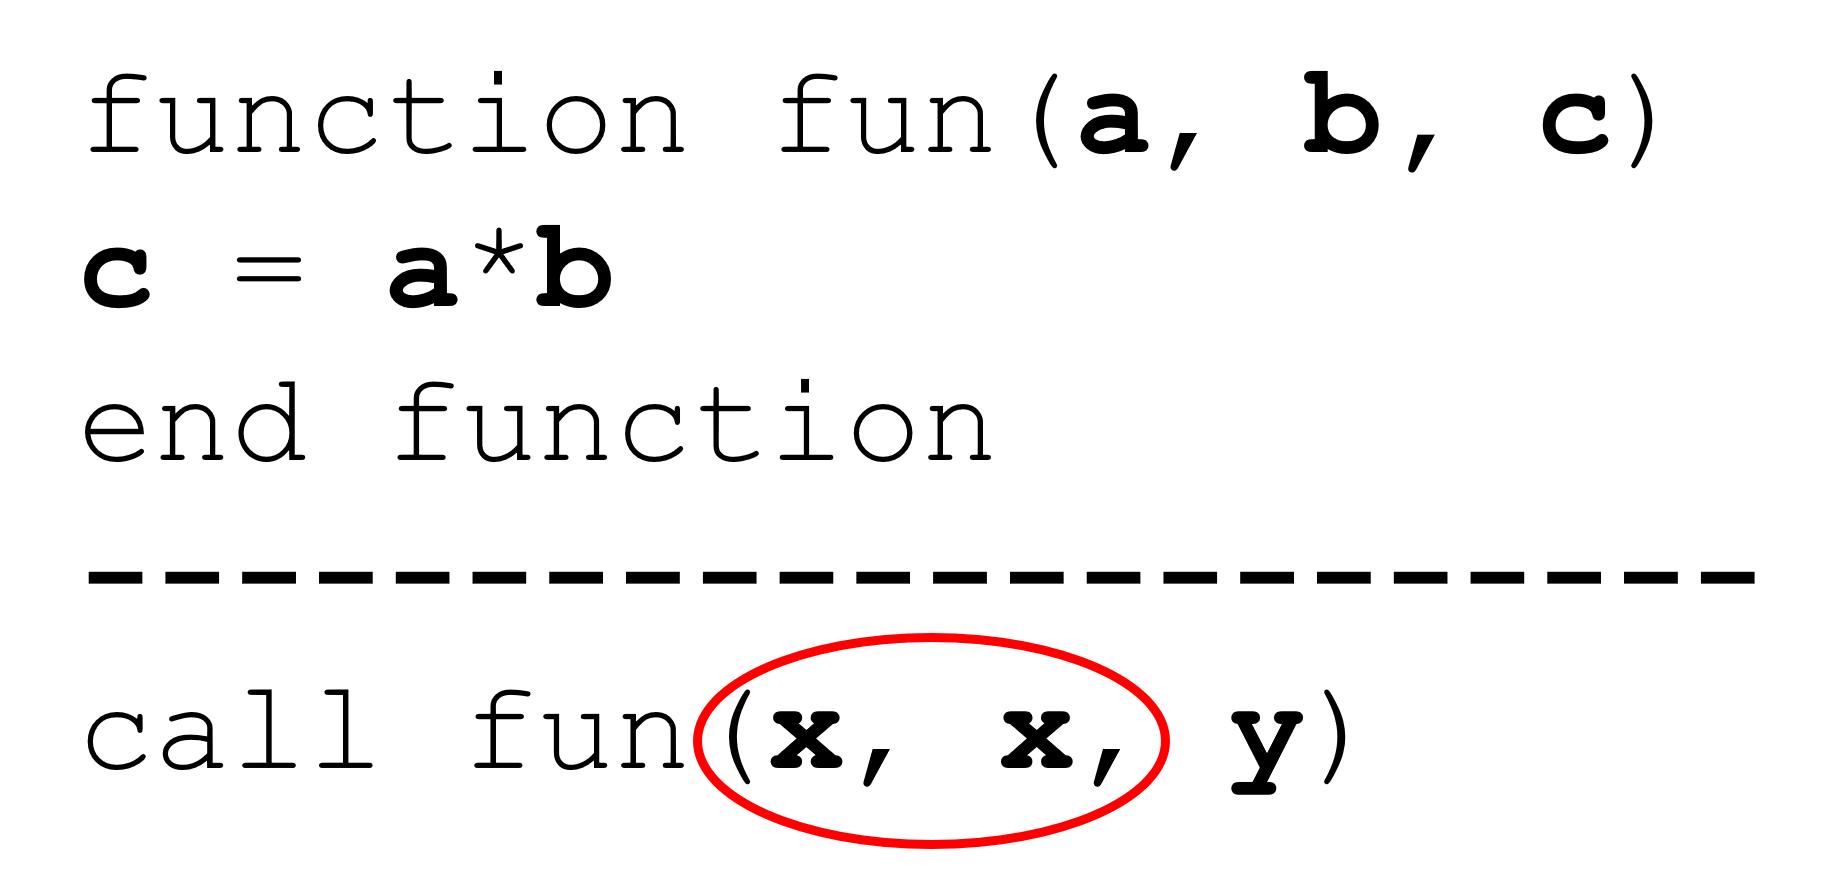
\includegraphics[width=60mm]{FiguresAD/aliasing1.png}}
		\subfigure{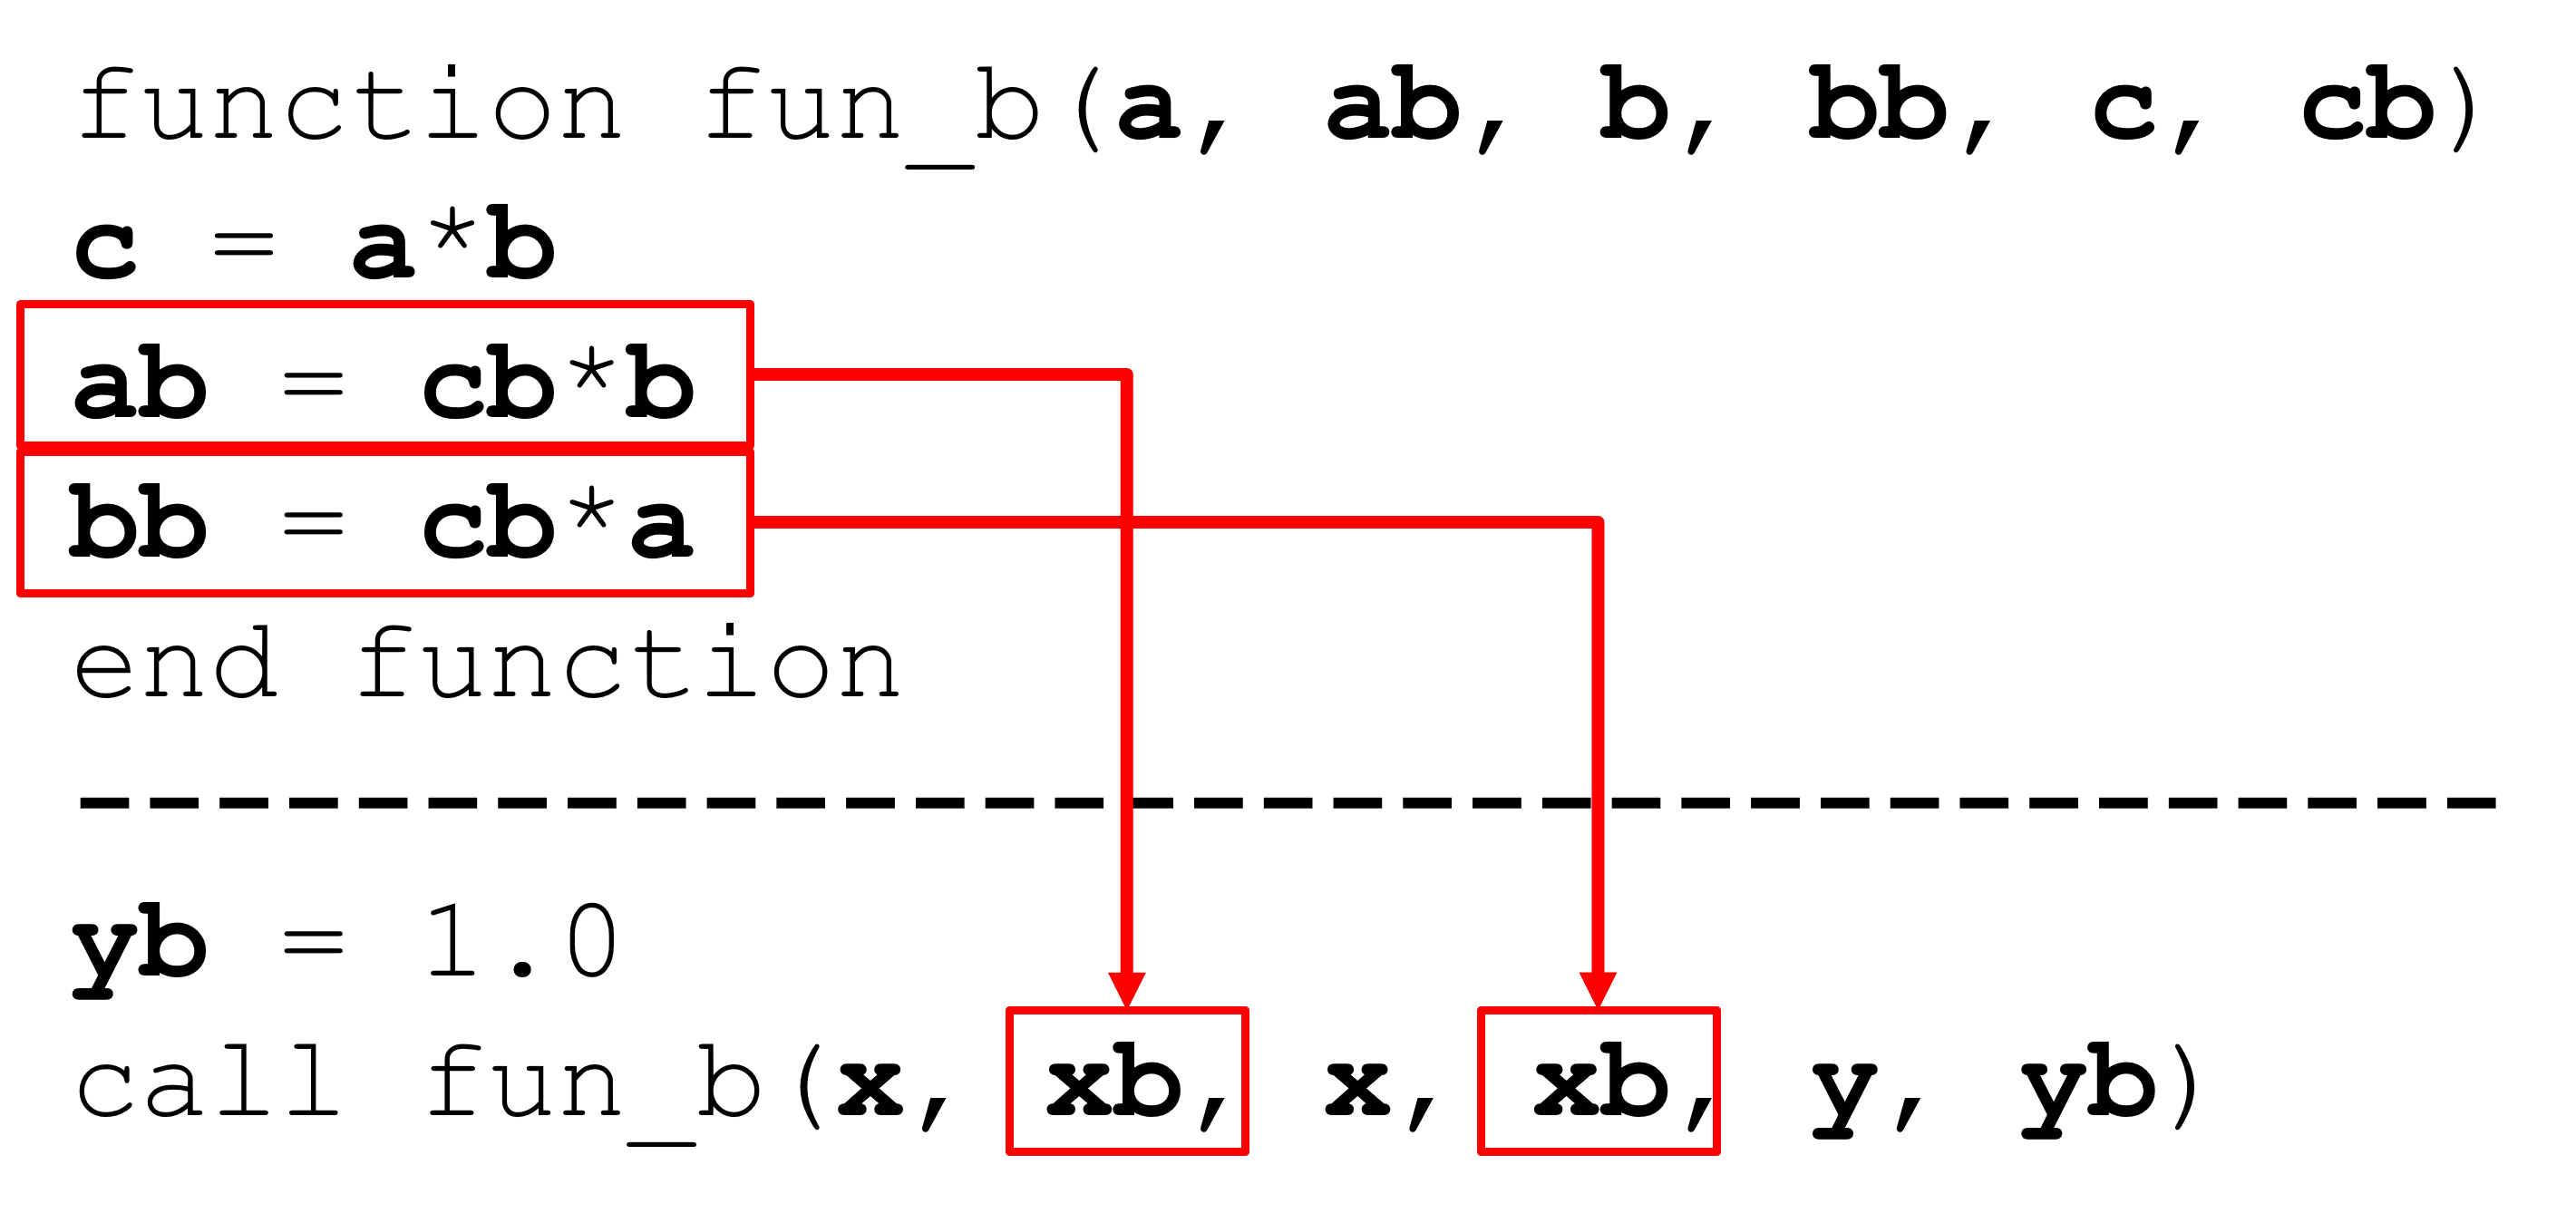
\includegraphics[width=60mm]{FiguresAD/aliasing2.png}}
		\caption{Example of issues with aliasing in adjoint AD.} \label{fig_alias}
	\end{figure}
	The aliasing happens when passing to the function the same variable {\tt x} to two formally separate arguments {\tt a} and {\tt b}. The correct adjoint for this specific call should be: {\tt xb = 2*x*yb}. However, since the same variable is passed when the routine is called, within {\tt fun\_b} the calculated {\tt ab} is passed to the first instance of {\tt xb}, while the calculated {\tt bb} is passed to the second instance. The order in which this is done determines the actual value of {\tt xb} but neither of the two is correct since it will overwrite, not sum to, the previous value!

	\item SIDE EFFECT: this issue happens again only in adjoint, when Tapenade needs to restore some SAVE'd variables within a certain routine. Such SAVE'd variables must therefore be visible in the calling routine, in order for Tapenade to checkpoint them before the call'ed routine and restore them after. Side effect variables are mentioned in the log file. An example is the case in which \textit{routine A} calls \textit{routine B}, and \textit{routine B} saves the variable \textit{ncall\_B} because it performs different actions depending on its value. As a result, Tapenade will ask that variable \textit{ncall\_B} is visible within \textit{routine A}. This can be solved for example using a module, as the dedicated {\tt b2mod\_ad} already available for this purposes, which defines and stores \textit{ncall\_B}, and is USE'd by both routines.

	\item ARRAY DIMENSIONS: in some cases Tapenade is not able to reconstruct the sizes of certain extra variables it has created during the differentiation. Often this happens when slicing of array is done in the primal code. In these cases it employs for the variable definition the size ``{\tt ISIZE1OFXXX}'', where {\tt XXX} is the variable name. In the automated script files some of these instances are already corrected using typical sizes like {\tt nCv, nFc}, etc. When differentiating the code, some of these may re-appear somewhere else. The user can look at the script files below in \ref{script_ad} to find inspiration to correct these.
\end{itemize}

%%%%%%%%%%%%%%%%%%%%%%%%%%%%%%%%%%%%%%%%%%%%%%%%%%%%%%%%%%%%%%%%%
%%%%%%%%%%%%%%%%%%%%%%%%%%%%%%%%%%%%%%%%%%%%%%%%%%%%%%%%%%%%%%%%%
\section{Detailed files description }\label{sec:description_files_ad}
%%%%%%%%%%%%%%%%%%%%%%%%%%%%%%%%%%%%%%%%%%%%%%%%%%%%%%%%%%%%%%%%%
%%%%%%%%%%%%%%%%%%%%%%%%%%%%%%%%%%%%%%%%%%%%%%%%%%%%%%%%%%%%%%%%%


	%%%%%%%%%%%%%%%%%%%%%%%%%%%%%%%%%%%%%%%%%%%%%%%%%%%%%%%%%%%%%%%%%
	\subsection{Description of pre-differentiated routines}
	%%%%%%%%%%%%%%%%%%%%%%%%%%%%%%%%%%%%%%%%%%%%%%%%%%%%%%%%%%%%%%%%%
	In this section additional information is given on the pre-differentiated routines available in {\tt B2.5/src/differentiation}. It is possible that with further code developments, the source code for some of the routines that have been duplicated and adapted will not be valid anymore, and as such should be modified

	\begin{description}
		\item{\tt b2mwqt\_diff.F} this routine is a copy of {\tt b2mwqt.F} used to write in output data concerning the numerical evolution of the diff'ed equations. The main difference wrt {\tt b2mwqt} is that here no checks on signs of quantities is done. {\tt b2mwqt\_diffv.F} is the same routine adapted also for multi-directional tangent differentiation

		\item{\tt b2mxac\_diff.F} this routine is a copy of {\tt b2mxac.F} and is used to evaluate the norm of the corrections. The difference wrt {\tt b2mxac.F} is that the type of the input variable {\tt dv} is {\tt B2Derivatives\_diff}. {\tt b2mxac\_diffv.F} is the same routine adapted also for multi-directional tangent differentiation

		\item{\tt b2mxar\_diff.F} this routine is a copy of {\tt b2mxar.F} and is used to evaluate the norm of the residuals. The difference wrt {\tt b2mxar.F} is that all sums are done using the absolute value of diff'ed quantities, since these can be negative and the use of {\tt sqrt} would fail. {\tt b2mxar\_diffv.F} is the same routine adapted also for multi-directional tangent differentiation

		\item{\tt b2uxus\_d.F} this routine solves a linear system of equations both for the primal and the derived quantities in tangent mode and is not a copy of {\tt b2uxus.F}. This pre-differentiated form of the linear solver is much more efficient than letting Tapenade differentiate throughout all the {\tt ilutern\_us\_solps} and {\tt b2mod\_ma28\_for\_us} routines. The theory behind is quite simple because tangent differentiating a linear system of equation of the form
		\begin{equation}
			Ax=b
		\end{equation}
		leads to the following results
		\begin{eqnarray}
			d(Ax)=d(b)\\
			\dot{A}x+A\dot{x}=\dot{b}\\
			A\dot{x}=\dot{b}-\dot{A}x
		\end{eqnarray}
		where $\dot{v}$ indicates the tangent derivative operator for the quantity $v$. The final system of equations makes use of the already known solution $x$ and solves for the unknown $\dot{x}$.	{\tt b2uxus\_dv.F} is the same routine adapted for multi-directional tangent differentiation

		\item{\tt b2uxus\_b.F} similar to the previous, but for adjoint AD. The routine solves te following equations:
		\begin{align}
			&A^T \overline{b} =  \overline{x},\\
			&\overline{A}_{i,j} = -x_j\overline{b}_i.
		\end{align}
		In this case, the first linear system is solved for $\overline{b}$ and simply transposing the matrix $A$. Afterwards, the primal linear system is solved and $x$ fed to the second equation.

		\item{\tt cond\_coef.F} this function is a copy of the same function present in {\tt heatdiff1D.F}. The reason it is put here is that Tapenade somehow produce a diff'ed {\tt heatdiff1D\_[db].F90} file that does not contain this subroutine

		\item{\tt dim\_[db].F90} this subroutine is a manual differentiation of the intrinsic function {\tt dim}. {\tt dim\_dv.F90} is the same routine adapted for multi-directional tangent differentiation

		\item{\tt erf\_[db].F} this subroutine is a manual differentiation of the intrinsic {\tt erf} which calculates the derivative of the error function as:
		\begin{equation}
			\frac{\partial erf}{\partial z}=\frac{2}{\sqrt{\pi}}e^{-z^2}
		\end{equation}
		{\tt erf\_dv.F} is the same routine adapted for multi-directional tangent differentiation

		\item{\tt read\_plasma\_state\_diff.F} and {\tt write\_plasma\_state\_diff.F} are copies of the same routines found in {\tt b2us\_plasma.F} with the only difference in the type of the input argument {\tt st}, which here is {\tt B2STATE\_DIFF}

		\item {\tt calc\_res\_fp\_diff.F} and {\tt  calc\_res\_fp\_multi.F}, these subroutines are used for the tangent/adjoint and tangent vector mode to calculate the maximum residual used in the adjoint fixed point iterator (see \ref{sec:run_adj})

		\item {\tt set\_adj\_gradient.F}, this routine is used by b2optim* routines to set and pass the gradient information from adjoint AD code to the optimization routines.

		\item {\tt set\_tgt\_perturbation.F}, this routine is used by b2optim* routines to set and pass the inpuit perturbation from the optimization routines to tangent AD code.

		\item {\tt set\_parameters.F }, this routine is added in the diff'ed version of {\tt b2mn\_step} within {\tt b2mod\_main} to assign the optimization parameters obtained from the optimization routines to the  input variables actually used by B2.5.

	\end{description}
	%%%%%%%%%%%%%%%%%%%%%%%%%%%%%%%%%%%%%%%%%%%%%%%%%%%%%%%%%%%%%%%%%
	\subsection{Description of script files}\label{script_ad}
	%%%%%%%%%%%%%%%%%%%%%%%%%%%%%%%%%%%%%%%%%%%%%%%%%%%%%%%%%%%%%%%%%
	In this section additional information is given on the script files used for or after the differentiation (available in {\tt \$SOLPSTOP/scripts}). Be aware that after modification of the source code some of the command lines in these scripts might not work anymore and thus the user has to modify them according to his needs.
	\begin{description}
		\item[collect\_tapenade\_files.sh]\index{collect\_tapenade\_files.sh} This scripts provides Tapenade with the name and path of the {\tt *.f} and {\tt *.f90} source files to be differentiated. These are automatically found in:\\ {\tt B2.5/builds/standalone.\$HOST\_NAME.\$COMPILER}. Such script also excludes specific files from the differentiation according to the {\tt excluded.txt} produced by calling the script {\tt exclude\_tapenade\_files.sh }

		\item[exclude\_tapenade\_files.sh] \index{exclude\_tapenade\_files.sh} this script produces the file {\tt excluded.txt} that lists all the files that have been excluded from the differentiation. Those are mainly the source files from {\tt B2.5/src/b2plot}, {\tt B2.5/src/convert}, {\tt B2.5/src/documentation}, \\{\tt B2.5/src/postprocessing}, {\tt B2.5/src/preprocessing} and {\tt B2.5/src/output}. Additionally, it allows to exclude/ignore/include specific source files according to these text files:
		\begin{description}
			\item{\tt B2.5/src/differentiation/files\_to\_exclude.txt}
			\item{\tt B2.5/src/differentiation/files\_to\_ignore.txt}
			\item{\tt B2.5/src/differentiation/files\_to\_keep.txt}
		\end{description}
		The difference among files to \textit{exclude} and to \textit{ignore} is that the latter are then used by postprocessing scripts that collect these files for compiling the diff'ed code.

		\item[postprocess\_tapenade\_tgt.sh]\index{postprocess\_tapenade\_tgt.sh} Script that automatically applies corrections to the diff'ed files obtained from Tapenade in tangent mode. It calls {\tt modify\_tapenade\_files\_d.sh}

		\item[postprocess\_tapenade\_tgt\_multi.sh]\index{postprocess\_tapenade\_tgt\_multi.sh} Script that automatically applies corrections to the diff'ed files obtained from Tapenade in tangent vector mode. It calls {\tt modify\_tapenade\_files\_d\_multi.sh}

		\item[postprocess\_tapenade\_adj.sh]\index{postprocess\_tapenade\_adj.sh} Script that automatically applies corrections to the diff'ed files obtained from Tapenade in adjoint mode. It calls {\tt modify\_tapenade\_files\_b.sh}

		\item[modify\_tapenade\_files\_d.sh]\index{modify\_tapenade\_files\_d.sh} This script modifies the diff'ed source files produced by Tapenade in tangent AD mode so that the diff'ed code can properly compile and run. The actions executed in the script are, among others:
		\begin{itemize}
			\item call the script {\tt move\_to\_F90.sh}

			\item call the script {\tt collect\_nodiff\_d.sh}

			\item removes the {\tt USE DIFFSIZES} statements in all routines since the needed sizes not known to Tapenade will be modified from the script

			\item Assign to some of the newly introduced variables the correct size, which Tapenade somehow cannot identify. These variables are normally easy to find by searching for the keyword {\tt ISIZE}. Others, located in {\tt b2mod\_driver\_diff.F90}, have been declared without any size or using wrong Fortran constructs. Note that this is the sequence that may change more likely with new code implementations or Tapenade releases

			\item some dummy variables of derived diff'ed type are somehow misinterpreted by Tapenade as pointers and thus nullified . Therefore these {\tt =>NULL()} statements are substituted with initialization to {\tt 0.0\_R8}.

			\item Remove the declaration of some functions which were hid to Tapenade but are actually visible through non-diff'ed files

			\item (SKIPPED: call the script {\tt remove\_initializations\_d.sh})

			\item Substitute the kind of (some) newly introduced variables from {\tt REAL} to {\tt REAL(KIND=R8)}. This is necessary for accurate gradient calculation

			\item Introduce some missing variables in the diff'ed {\tt MAPPING} type

			\item introduce a {\tt B2DIAGNOSTIC} type for the diff'ed plasma state

			\item Copy from {\tt \$TAPENADEDIR} the two additional source files needed for the context verification procedure
		\end{itemize}

		\item[move\_to\_F90.sh]\index{move\_to\_F90.sh} Changes the diff'ed files extensions from {\tt .f90} to {\tt .F90}. This is needed by the compilations rules within the B2.5 Makefile.

		\item[collect\_nodiff\_d.sh]\index{collect\_nodiff\_d.sh} Collect source files that have not been diff'ed and make sure the modules used in such files are the diff'ed ones. At this stage also the name of the diff'ed modules is changed by substituting the {\tt \_d} in their name with {\tt \_diff}, which makes it easier to compile.

		\item[remove\_initializations\_d.sh]\index{remove\_initializations\_d.sh} In {\tt b2mod\_driver\_diff.F90} Tapenade puts the initialization of some diff'ed variables to {\tt 0.0\_R8}. Among these, also diff'ed plasma state variables as for example {\tt state\%pl\%te} are initialized. However, when run continuation is enabled, such initializations would overwrite the data read from {\tt b2fdiffi}. Therefore, this script looks for which plasma state variables are read in {\tt read\_plasma\_state\_diff.F} and makes sure that if they initialization in {\tt b2mod\_driver\_diff.F90} is removed.

		\item[modify\_tapenade\_files\_d\_multi.sh]\index{modify\_tapenade\_files\_d\_multi.sh} This script modifies the diff'ed source files produced by Tapenade in tangent vector mode so that the diff'ed code can properly compile and run. The actions executed in the script are similar to what is done in {\tt modify\_tapenade\_files\_d.sh}.

		\item[collect\_nodiff\_d\_multi.sh]\index{collect\_nodiff\_d\_multi.sh} Called within {\tt modify\_tapenade\_files\_d\_multi.sh} and executes similar commands as {\tt collect\_nodiff\_d.sh}.

		\item[modify\_tapenade\_files\_b.sh]\index{modify\_tapenade\_files\_b.sh} This script modifies the diff'ed source files produced by Tapenade in adjoint mode so that the diff'ed code can properly compile and run. The actions executed in the script are similar to what is done in {\tt modify\_tapenade\_files\_d.sh}.

		\item[collect\_nodiff\_b.sh]\index{collect\_nodiff\_b.sh} Called within {\tt modify\_tapenade\_files\_b.sh} and executes similar commands as \\{\tt collect\_nodiff\_d.sh}.

		\item[collect\_nodiff\_p.sh]\index{collect\_nodiff\_p.sh} Executes similar commands as {\tt collect\_nodiff\_d.sh}, can be used collect files when the pre-processing mode of Tapenade is used
	\end{description}
